\documentclass[../main.tex]{subfiles}

\begin{document}
\setcounter{chapter}{0}
\chapter{运算器组成实验}

\section{实验目的}

\begin{enumerate}

    \item 熟悉双端口通用寄存器组的读写操作;

    \item 熟悉运算器的数据传送通路;

    \item 验证74LS181的加、减、与、或功能;

    \item 按给定的数据, 完成几种指定的算术、逻辑运算运算.

\end{enumerate}

\section{实验内容}

\begin{enumerate}

    \item 用微程序模式进行相应的运算;

    \item 在独立模式下对 A=F0H, B=10H 进行加、减、与、或运算.

\end{enumerate}

\section{实验过程}

\subsection{微程序模式}

\begin{enumerate}

    \item 打开仿真软件, 选择微程序模式, 打开DP、SWA、SWC开关后启动电源, 进行运算器实验.

    \item 按下QD按钮, 观察到SBUS控制信号灯亮起. 此时从数据开关输入实验数据. (如图 \ref{fig:1.1} 所示.)

          \begin{figure}[hp]
              \centering
              \subfigure[输入A]{
                  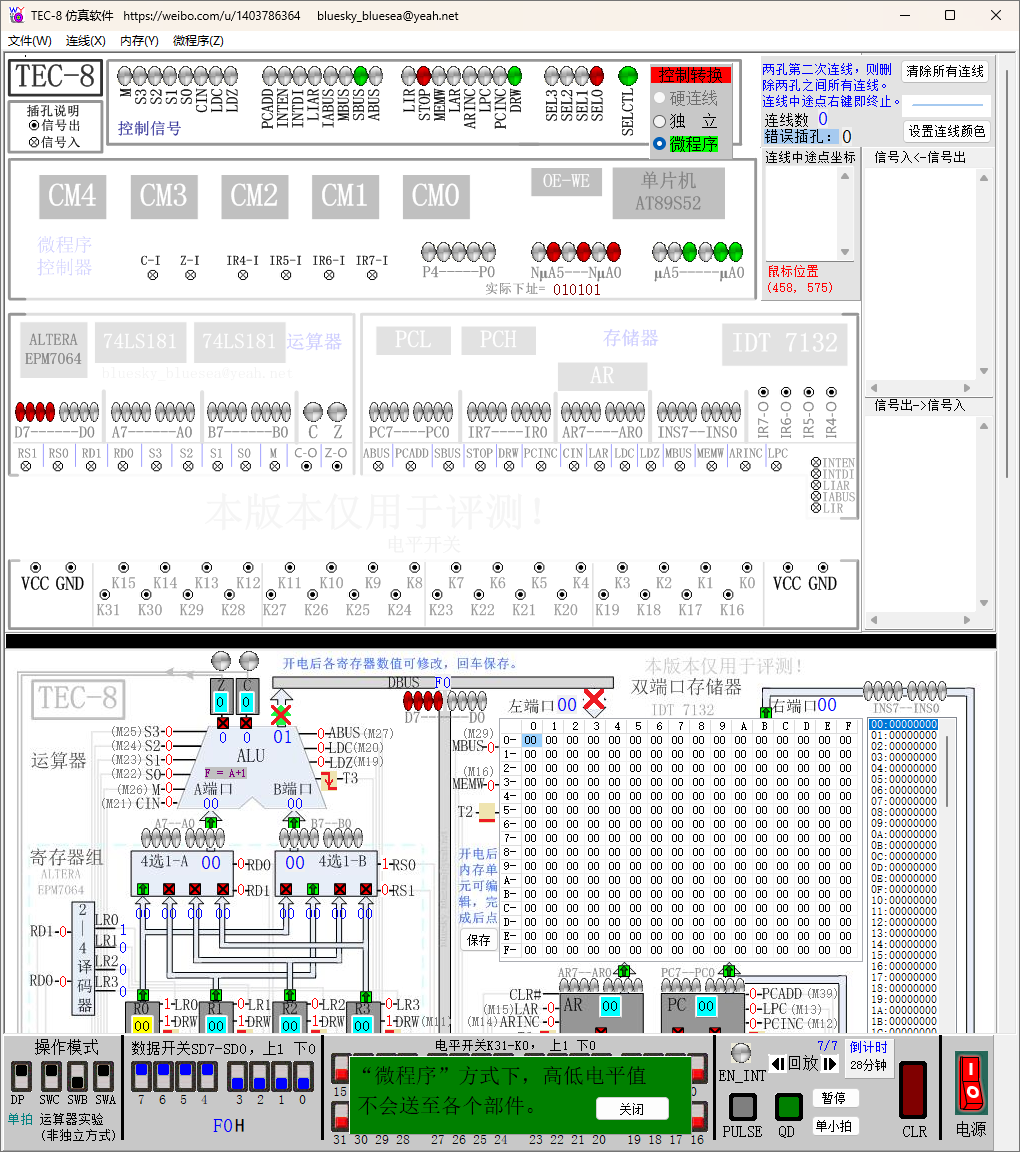
\includegraphics[width=0.3\textwidth]{screenshots/1.1.1.2.png}
              }
              \subfigure[输入B]{
                  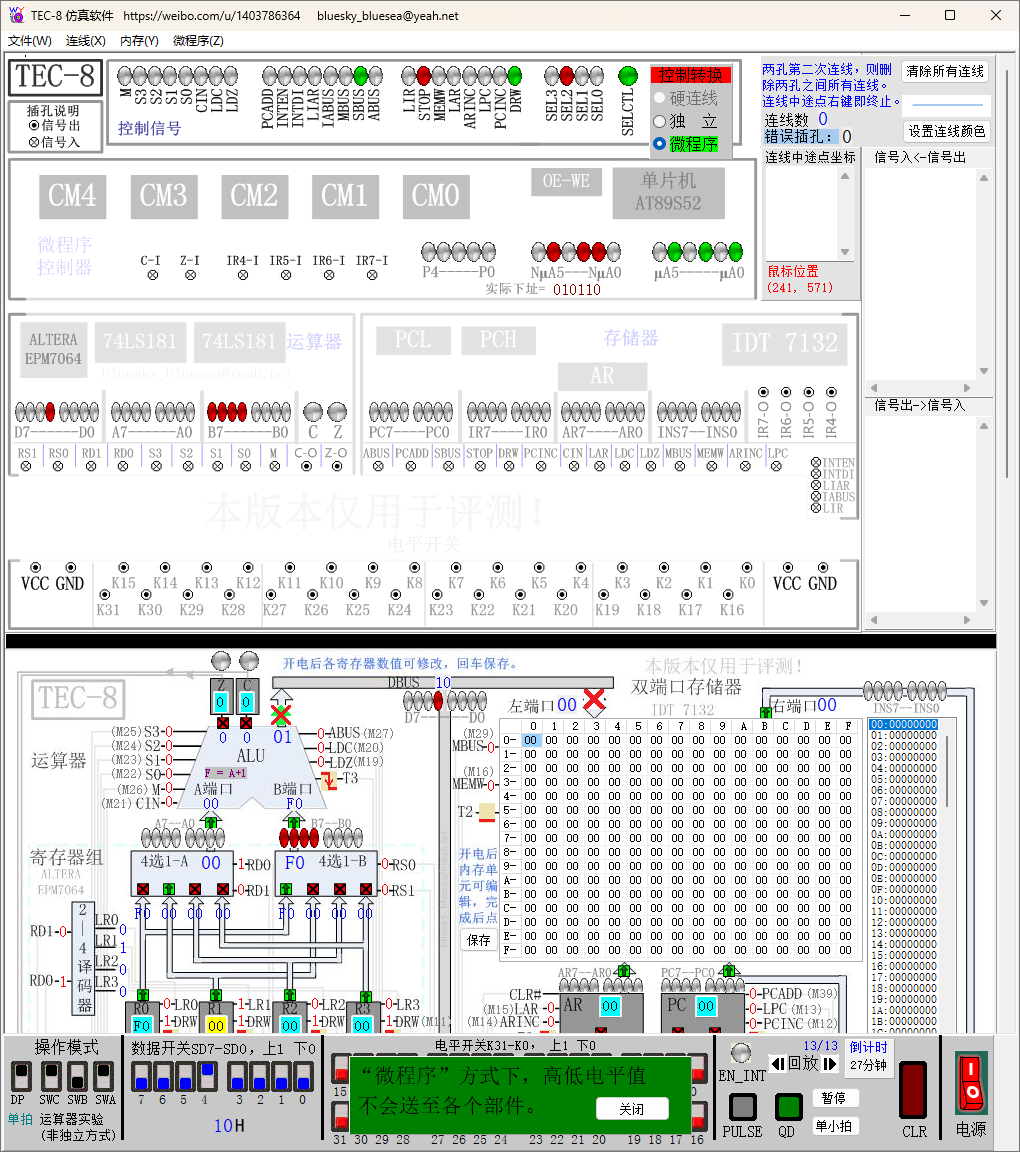
\includegraphics[width=0.3\textwidth]{screenshots/1.1.1.3.png}
              }
              \caption{输入数据 (微程序)}
              \label{fig:1.1}
          \end{figure}

    \item 按下QD按钮4次, 依次进行加、减、与、非运算, 观察并记录实验结果. (如图 \ref{fig:1.2} 所示.)

          \begin{figure}[hp]
              \centering
              \subfigure[加法运算]{
                  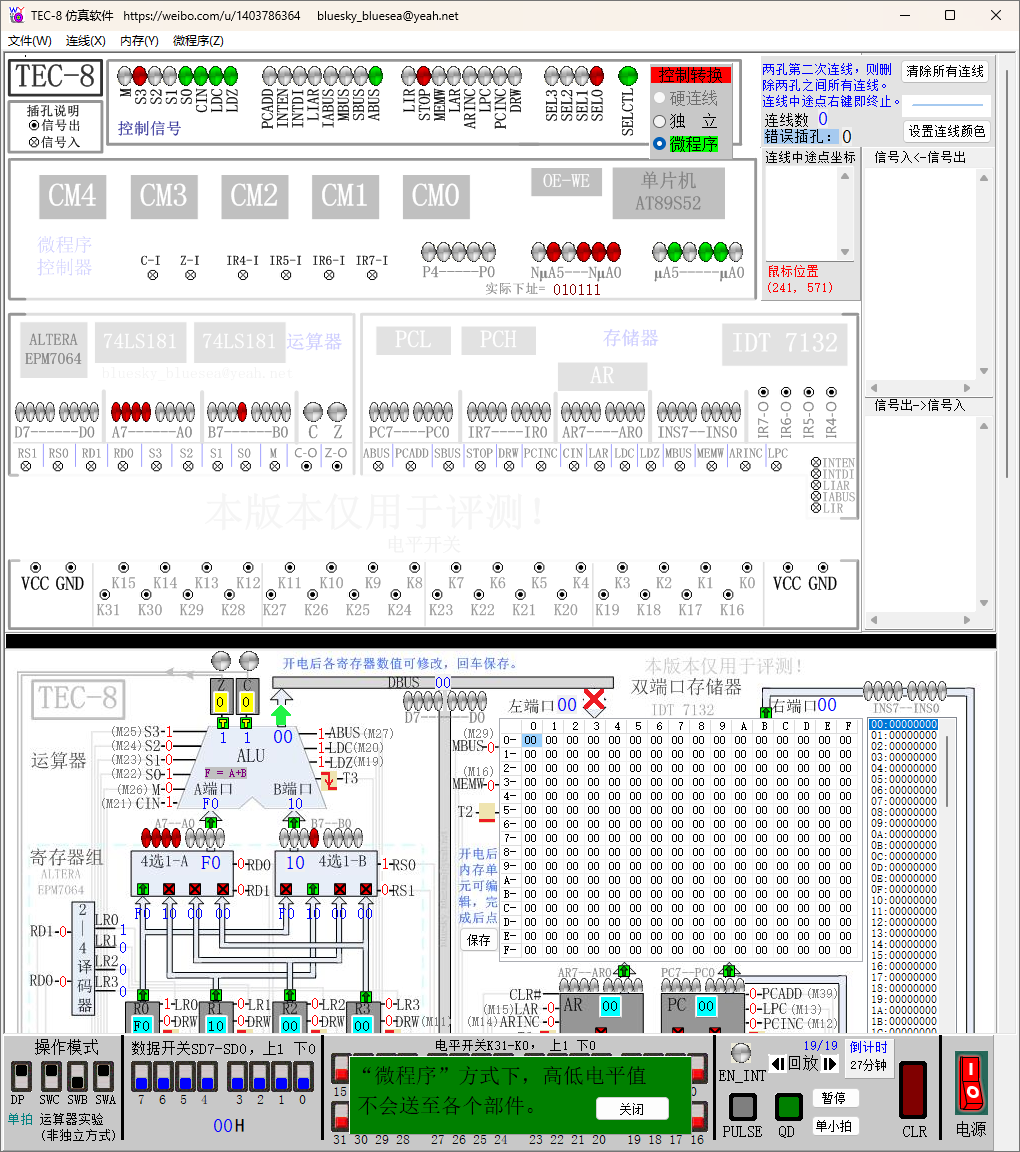
\includegraphics[width=0.3\textwidth]{screenshots/1.1.1.4.png}
              }
              \subfigure[减法运算]{
                  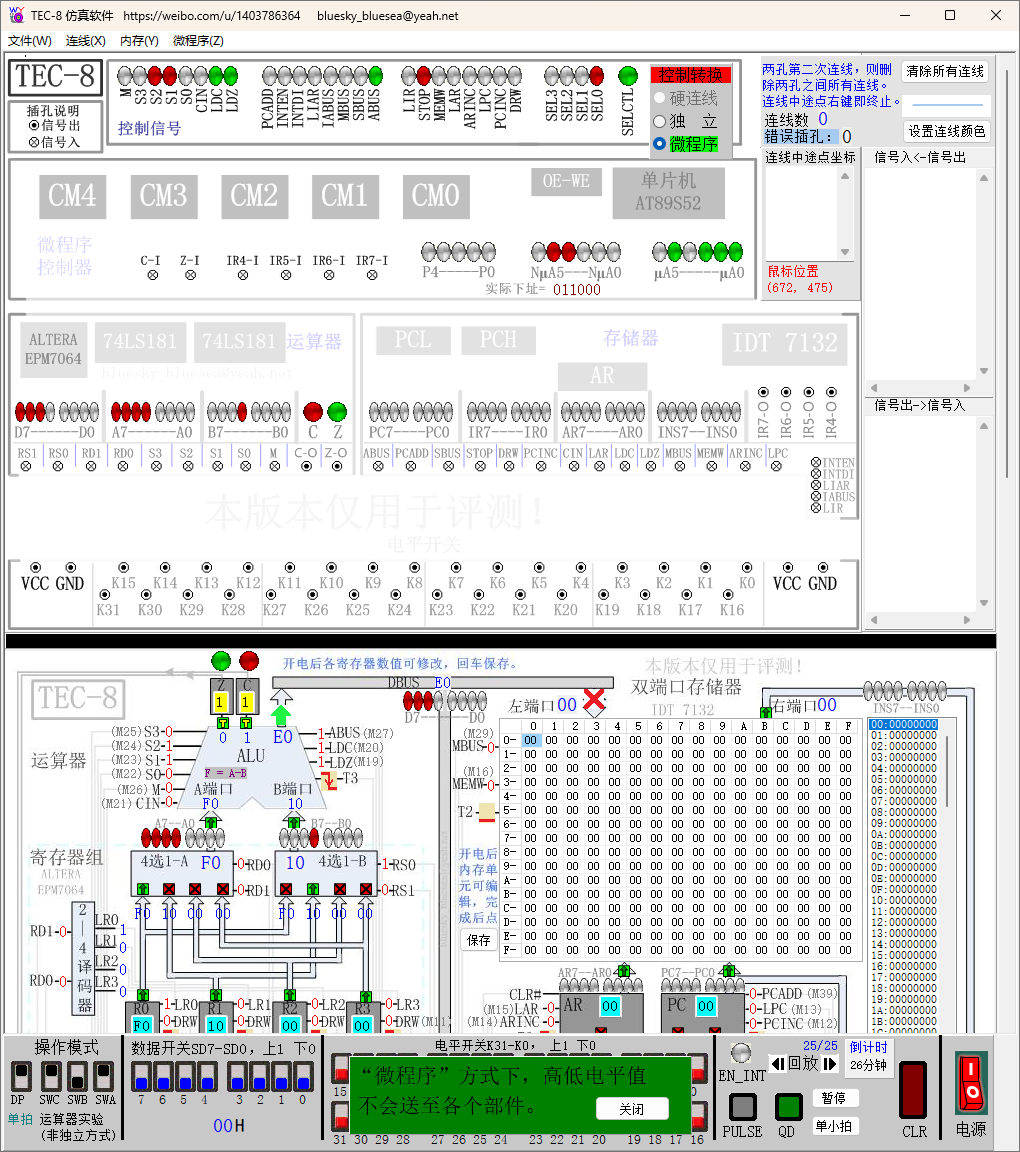
\includegraphics[width=0.3\textwidth]{screenshots/1.1.1.5.png}
              }
              \\
              \subfigure[与运算]{
                  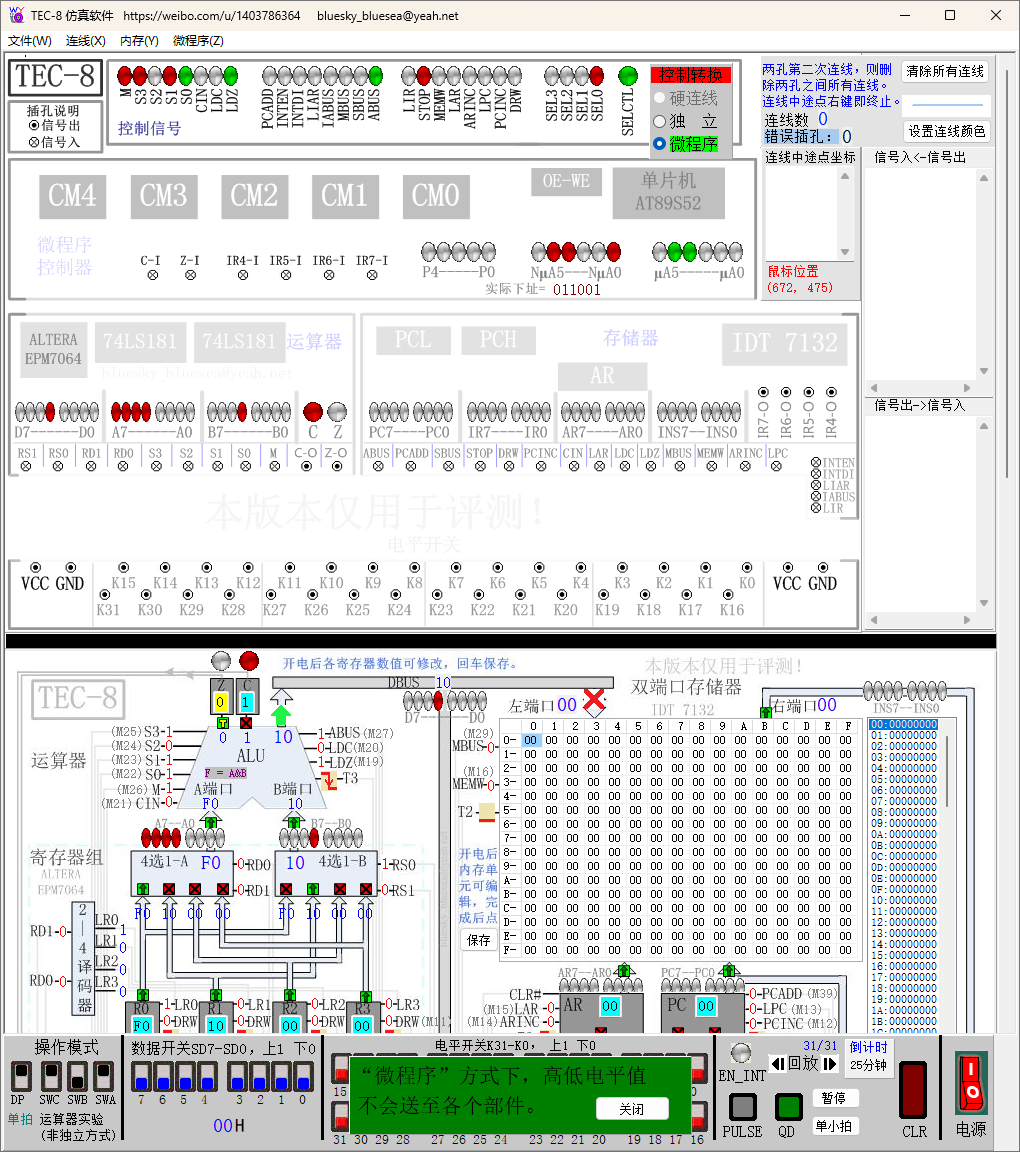
\includegraphics[width=0.3\textwidth]{screenshots/1.1.1.6.png}
              }
              \subfigure[或运算]{
                  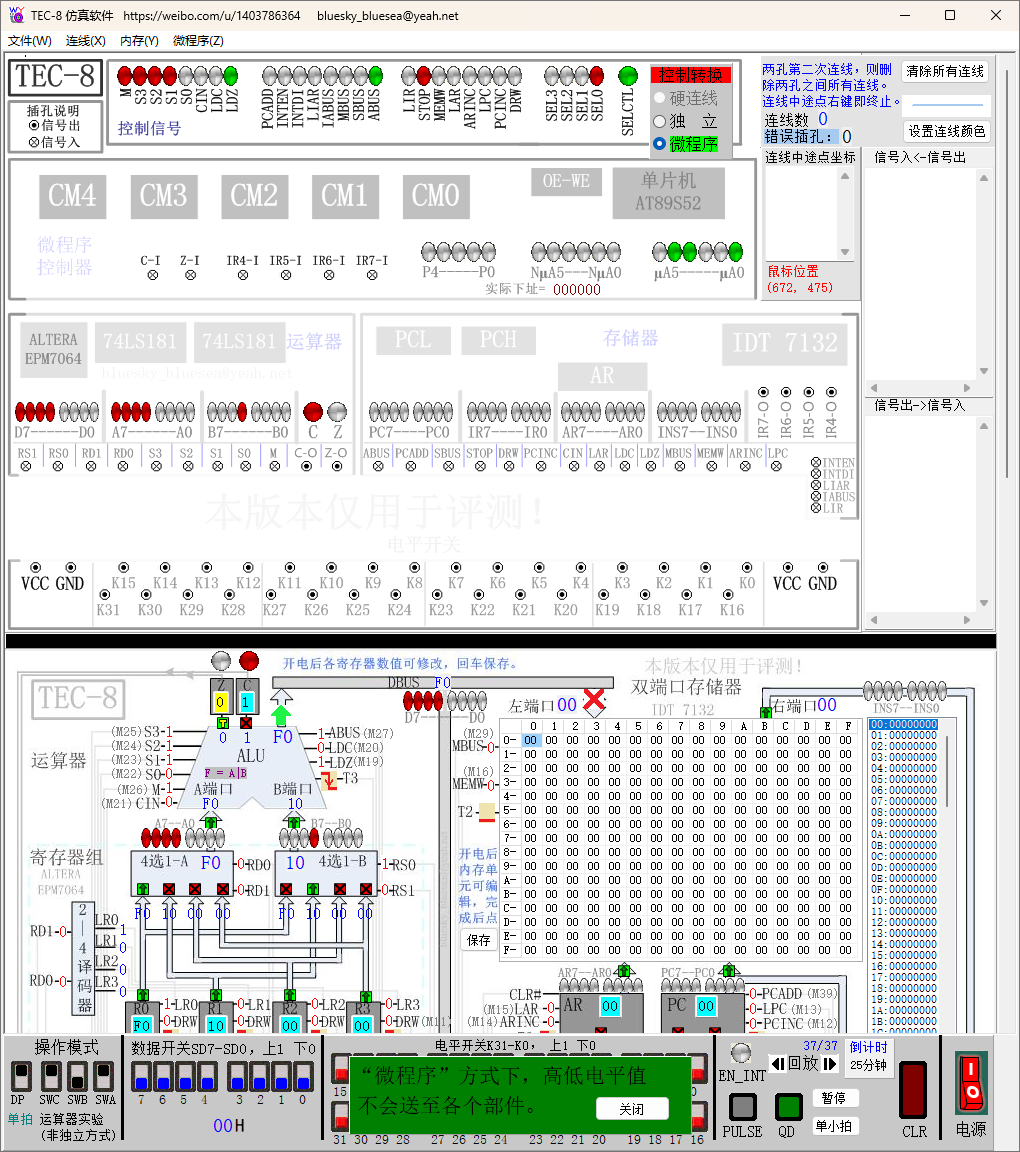
\includegraphics[width=0.3\textwidth]{screenshots/1.1.1.7.png}
              }
              \caption{运算结果 (微程序)}
              \label{fig:1.2}
          \end{figure}

    \item 重复上述步骤, 每次输入不同的实验数据, 观察实验结果并记录汇总. (如表 \ref{tab:1.1} 所示.)

          \begin{table}[htb]
              \centering
              \begin{tabular}{cc|cccccccccccc}
                  \Xhline{1pt}
                  \multicolumn{2}{c|}{实验数据} & \multicolumn{12}{c}{实验结果}                                                                                                                                                                                  \\ \hline
                  \multirow{2}{*}{数A}       & \multirow{2}{*}{数B}       & \multicolumn{3}{c|}{加} & \multicolumn{3}{c|}{减} & \multicolumn{3}{c|}{与} & \multicolumn{3}{c}{或}                                                                               \\
                                            &                           & 数据                     & C                      & \multicolumn{1}{c|}{Z} & 数据                    & C & \multicolumn{1}{c|}{Z} & 数据  & C & \multicolumn{1}{c|}{Z} & 数据  & C & Z \\ \hline
                  F0H                       & 10H                       & 00H                    & 1                      & \multicolumn{1}{c|}{1} & E0H                   & 1 & \multicolumn{1}{c|}{0} & 10H & / & \multicolumn{1}{c|}{0} & F0H & / & 0 \\
                  FFH                       & AAH                       & A9H                    & 1                      & \multicolumn{1}{c|}{0} & 55H                   & 1 & \multicolumn{1}{c|}{0} & AAH & / & \multicolumn{1}{c|}{0} & FFH & / & 0 \\
                  10H                       & F0H                       & 00H                    & 1                      & \multicolumn{1}{c|}{1} & 20H                   & 0 & \multicolumn{1}{c|}{0} & 10H & / & \multicolumn{1}{c|}{0} & F0H & / & 0 \\
                  55H                       & AAH                       & FFH                    & 0                      & \multicolumn{1}{c|}{0} & ABH                   & 0 & \multicolumn{1}{c|}{0} & 00H & / & \multicolumn{1}{c|}{1} & FFH & / & 0 \\
                  \Xhline{1pt}
              \end{tabular}
              \caption{实验结果 (微程序)}
              \label{tab:1.1}
          \end{table}

\end{enumerate}

\subsection{独立模式}

\begin{enumerate}

    \item 完成实验相关连线 (如图 \ref{fig:1.3} 所示), 并打开 DP 开关, 开启电源.

          \begin{figure}[hp]
              \centering
              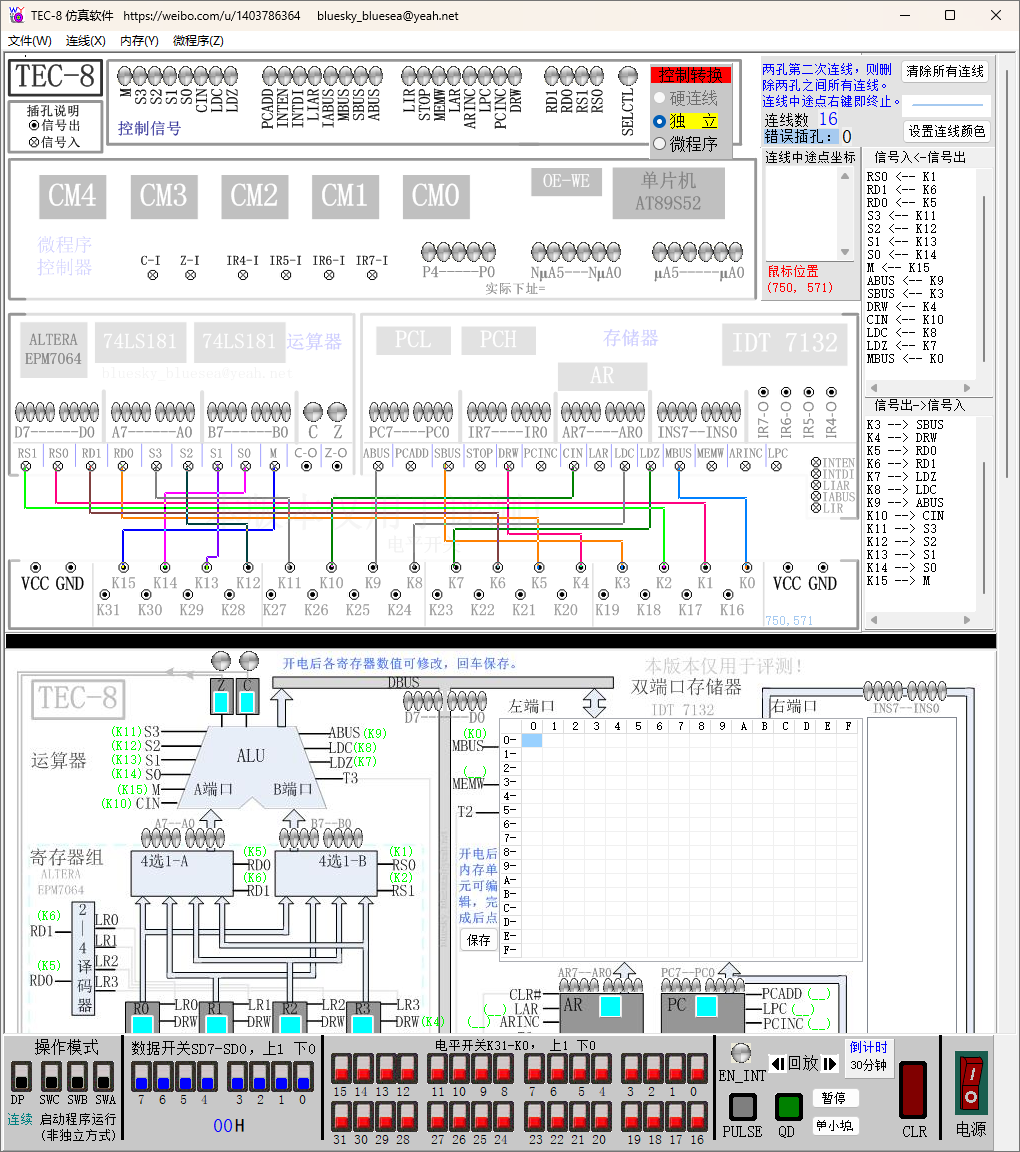
\includegraphics[width=0.3\textwidth]{screenshots/1.2.1.png}
              \caption{连线 (独立)}
              \label{fig:1.3}
          \end{figure}

    \item 将数据A (F0H) 与数据B (10H) 分别输入寄存器R$_0$, R$_1$中. (如图 \ref{fig:1.4} 所示.)

          \begin{figure}[hp]
              \centering
              \subfigure[输入A]{
                  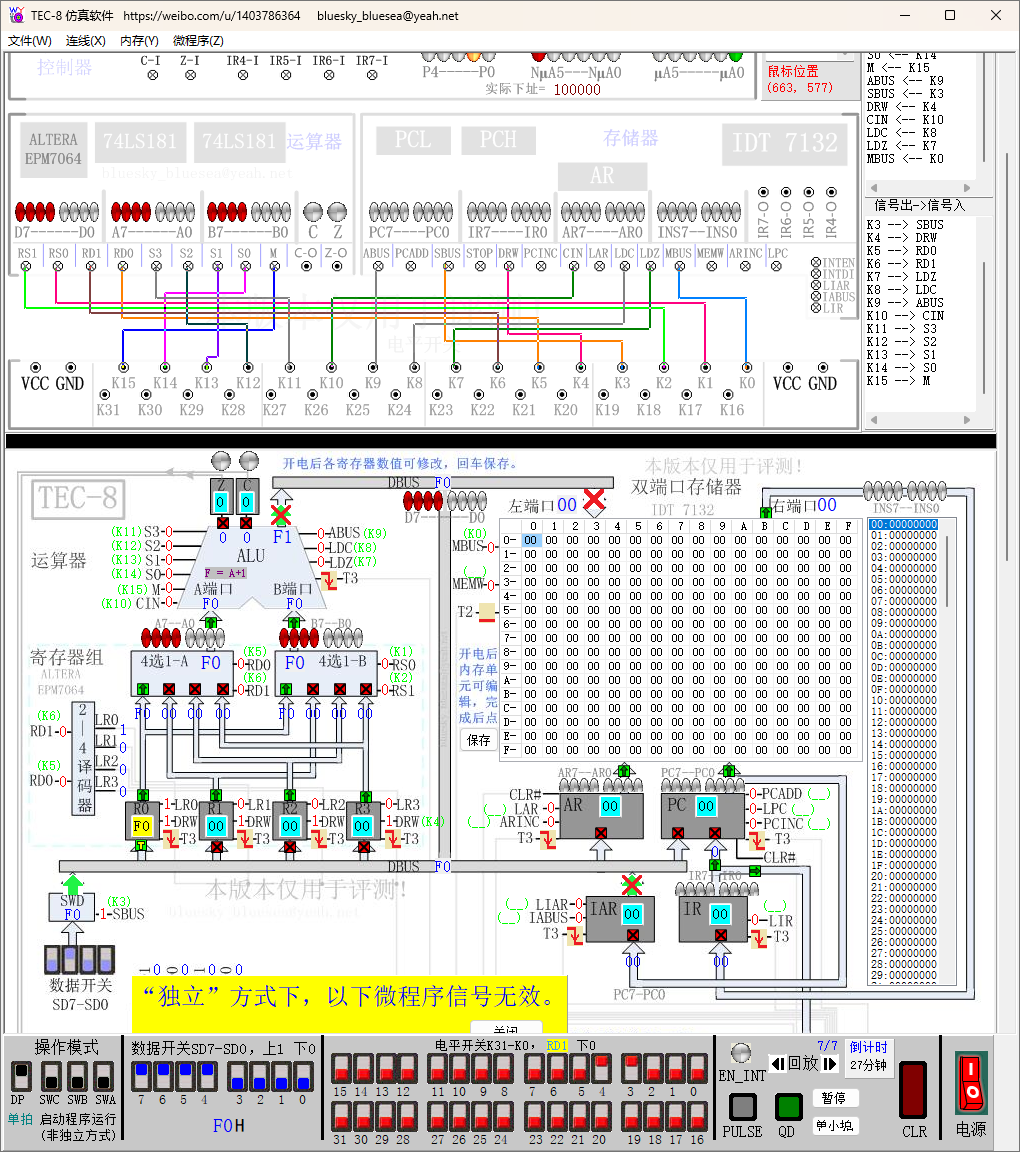
\includegraphics[width=0.3\textwidth]{screenshots/1.2.2.png}
              }
              \subfigure[输入B]{
                  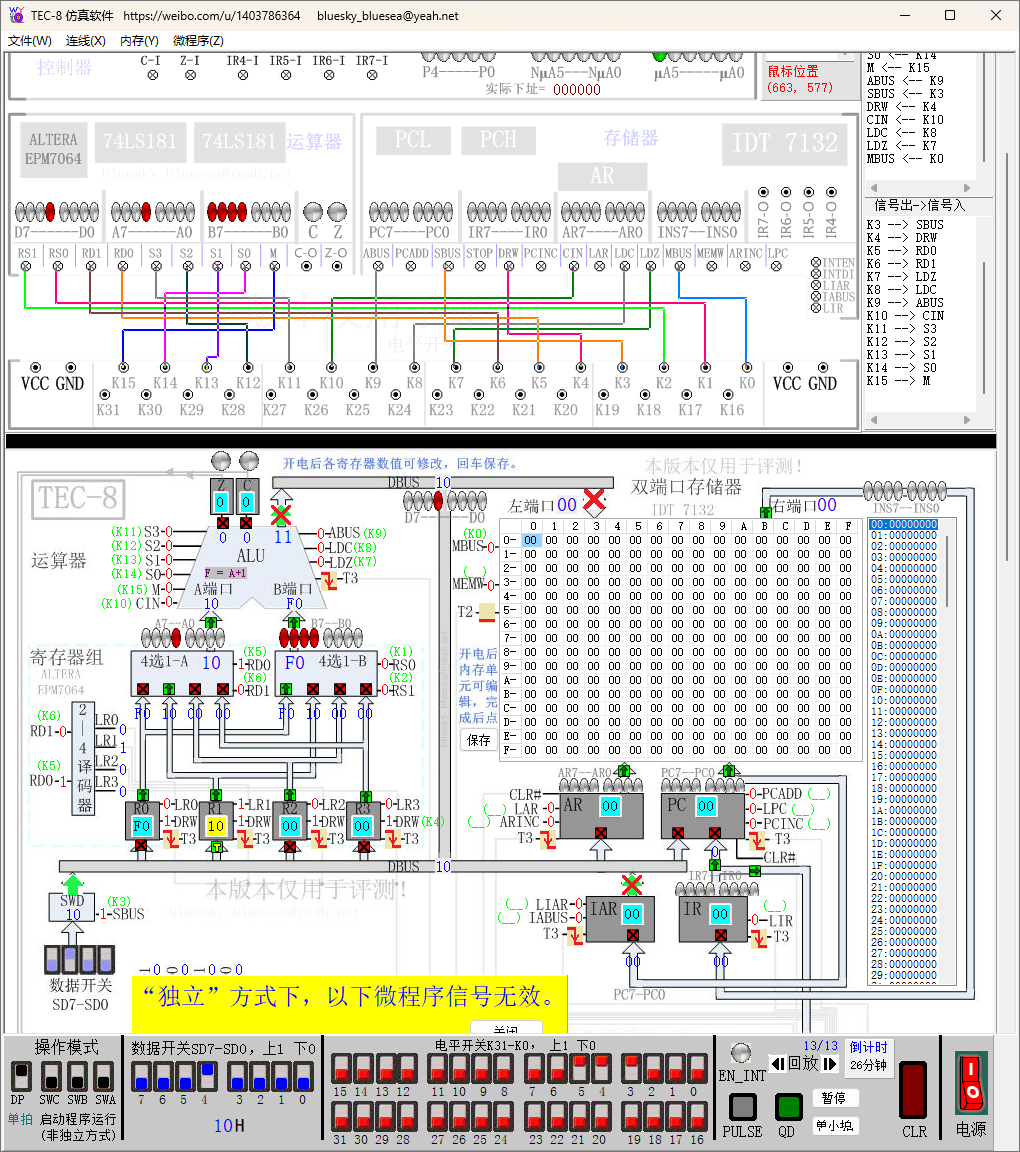
\includegraphics[width=0.3\textwidth]{screenshots/1.2.3.png}
              }
              \caption{输入数据 (独立)}
              \label{fig:1.4}
          \end{figure}

    \item 关闭SBUS与DRW对应的开关, 使得数据开关不再进行总线的输入且总线上的数据不再写入寄存器.
          控制RS$_0$打开, RS$_1$, RD$_0$, RD$_1$ 关闭, 使ALU的A, B两个端口分别输入R$_0$, R$_1$中的数据.
          调整 ALU 的控制信号使其进行加法运算, 观察其运算结果.

          % \begin{figure}[hp]
          %     \centering
          %     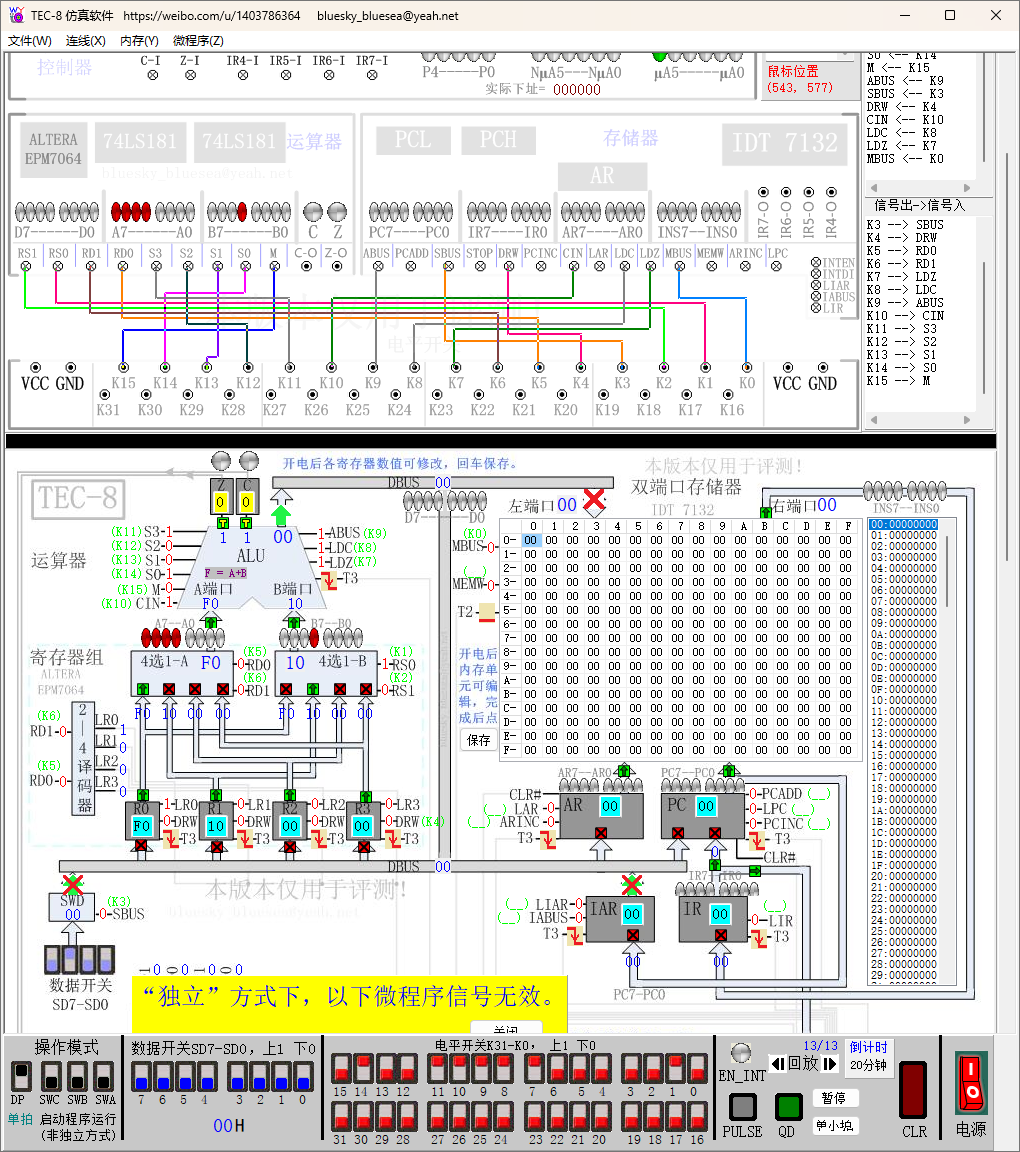
\includegraphics[width=0.3\textwidth]{screenshots/1.2.4.png}
          %     \caption{加法运算 (独立)}
          %     \label{fig:1.5}
          % \end{figure}

    \item 继续调整 ALU 的控制信号, 使其依次做减、与、或运算, 观察实验结果. (如图 \ref{fig:1.5} 所示.)

          \begin{figure}[hp]
              \centering
              \subfigure[加法运算]{
                  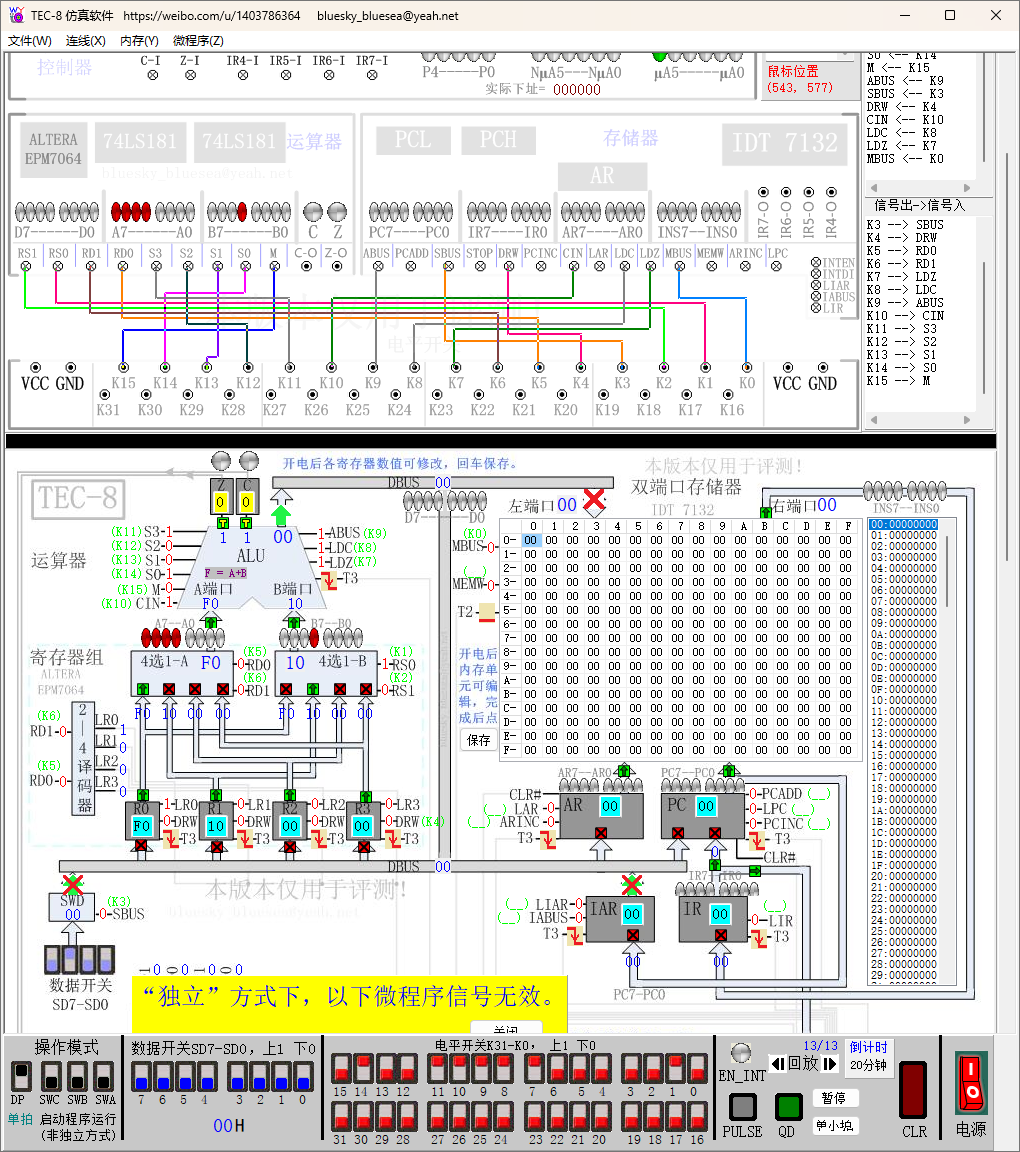
\includegraphics[width=0.3\textwidth]{screenshots/1.2.4.png}
              }
              \subfigure[减法运算]{
                  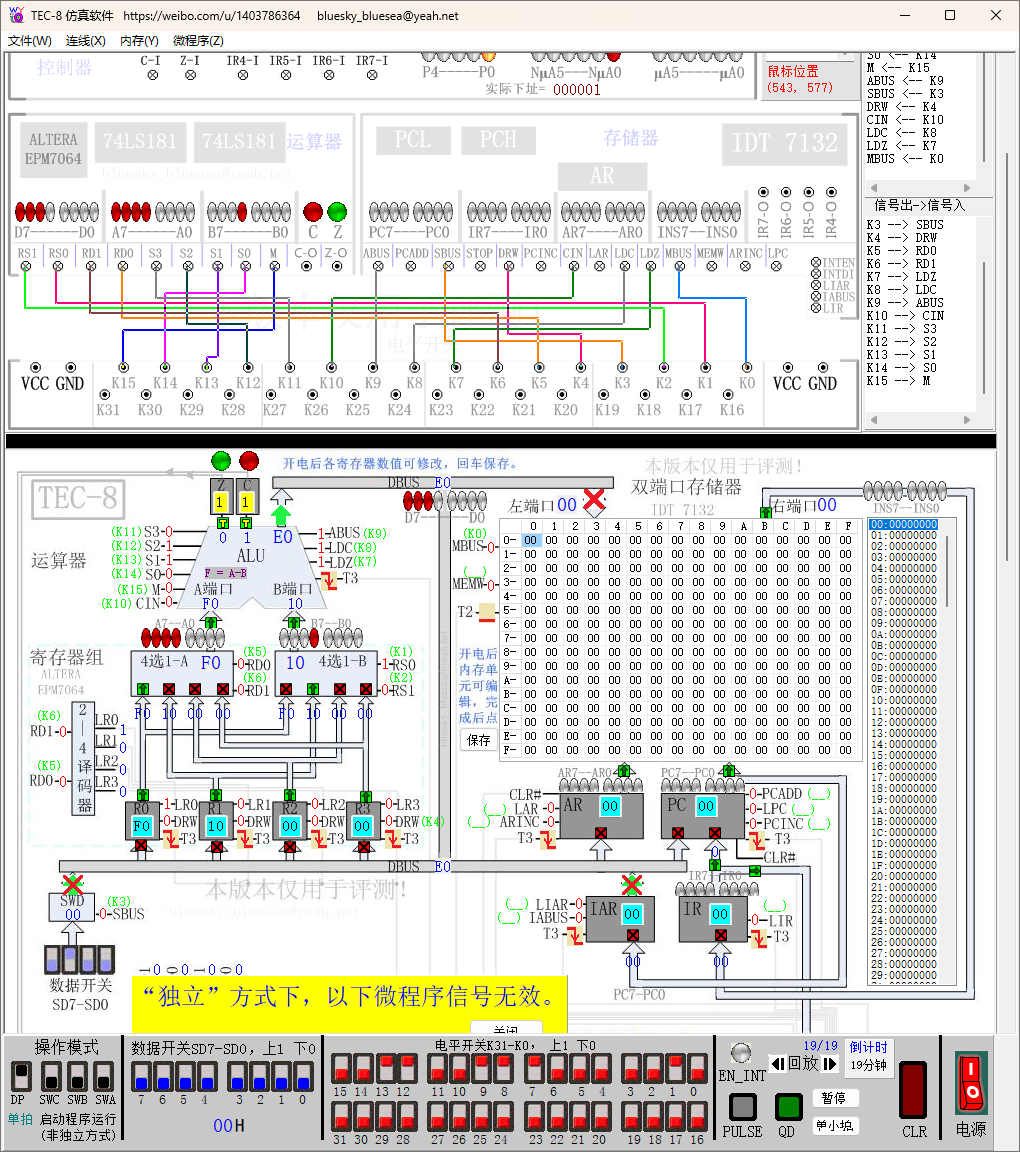
\includegraphics[width=0.3\textwidth]{screenshots/1.2.5.png}
              }
              \\
              \subfigure[与运算]{
                  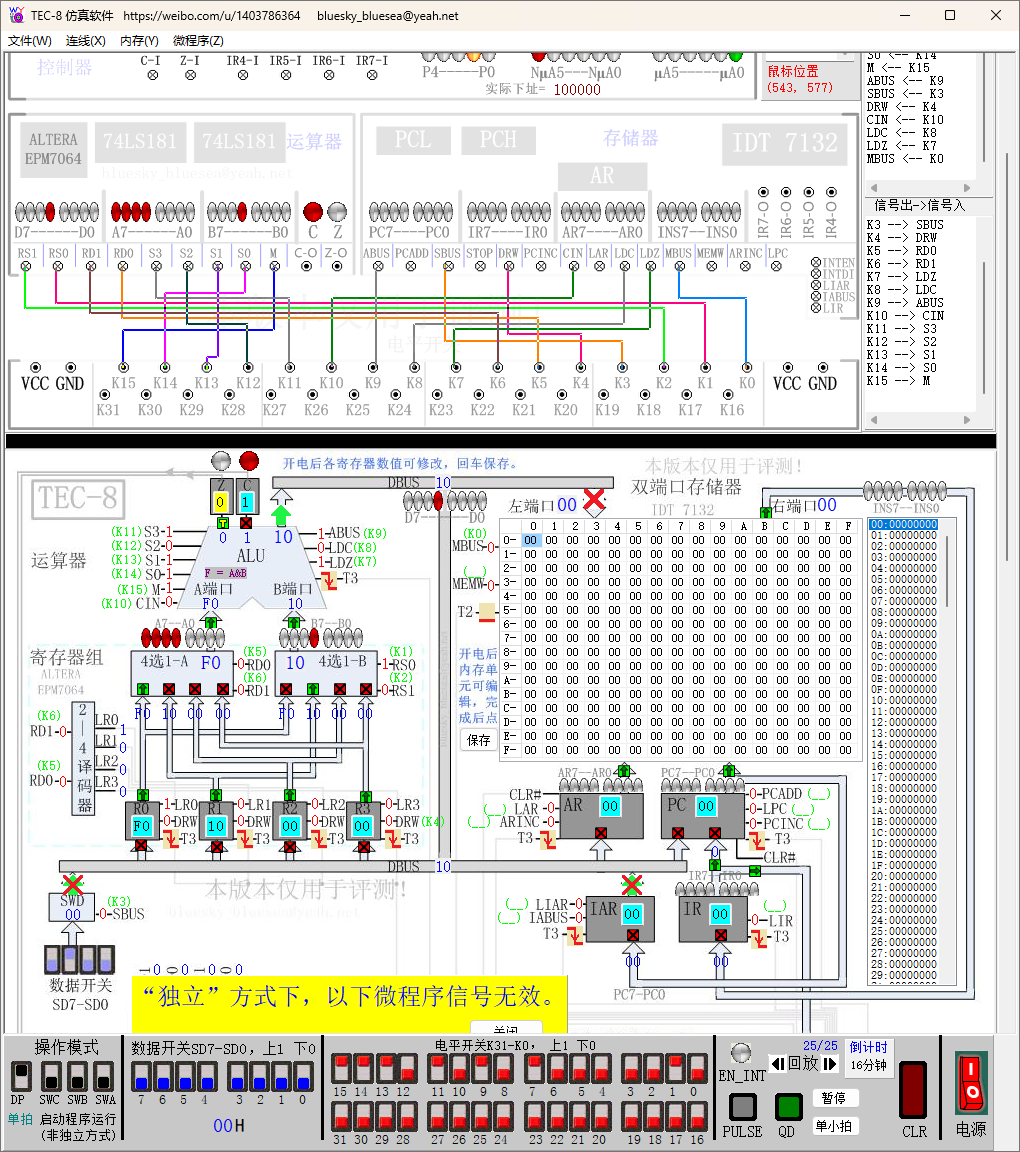
\includegraphics[width=0.3\textwidth]{screenshots/1.2.6.png}
              }
              \subfigure[或运算]{
                  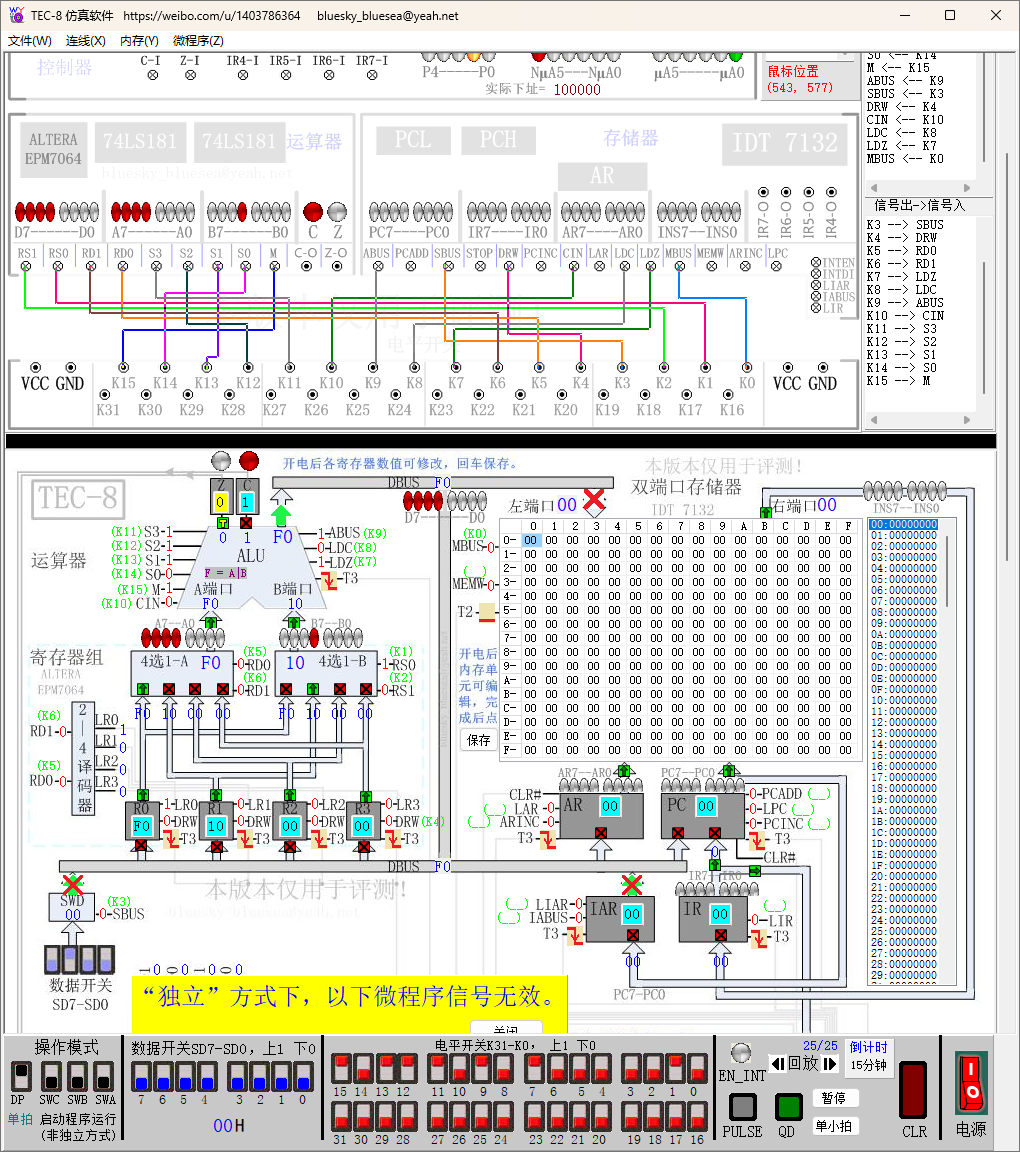
\includegraphics[width=0.3\textwidth]{screenshots/1.2.7.png}
              }
              \caption{运算结果 (独立)}
              \label{fig:1.5}
          \end{figure}

    \item 记录并整理实验结果. (如表 \ref{tab:1.2} 所示.)

          \begin{table}[htb]
              \centering
              \begin{tabular}{cccc}
                  \Xhline{1pt}
                  运算类型 & 数据结果 & C & Z \\ \hline
                  加    & 00H  & 1 & 1 \\
                  减    & E0H  & 1 & 0 \\
                  与    & 10H  & / & 0 \\
                  或    & F0H  & / & 0 \\
                  \Xhline{1pt}
              \end{tabular}
              \caption{实验结果 (独立)}
              \label{tab:1.2}
          \end{table}

\end{enumerate}

\section{思考与心得}

\subsection{思考}

\subsubsection{实验中各个信号的作用}

\begin{itemize}

    \item M, S$_{0 - 3}$, CIN

          用于在进行运算时控制 ALU 执行相应的运算操作 (可通过 74LS181 功能表查得). 在ALU执行运算的步骤中必需, 在其他步骤中非必需.

    \item LDC, LDZ

          分别用于在进行运算时控制 ALU 的进位标志与结果为0标志是否进行输出. 在算术运算下一般全开启, 在逻辑运算下可不开启LDC, 在其他步骤中非必需.

    \item SEL$_{0 - 3}$

          在输入数据时, 控制输入的数据送入哪个寄存器; 在进行运算时, 控制操作数A, B分别从哪个寄存器获得. 本实验中,全程都须确保这些信号的正确性.

    \item DRW, SBUS

          前者控制寄存器能否从DBUS写入数据, 后者控制数据开关的信号能否送入 DBUS. 在向寄存器中写入数据时两者需要开启; 在其他步骤中需要关闭DRW, SBUS非必需.

\end{itemize}

\subsubsection{ALU 具有记忆功能吗? 如果有, 如何设计?}

74LS181 本身不具有记忆功能. 但是, 配合寄存器, 可以令ALU的F端口始终输出某一特定寄存器的值, 实现类似记忆的功能.

\subsubsection{为什么在 ALU 的 A 端口和 B 端口的数据确定后, 在数据总线 DBUS 上能够直接观测运算的数据结果, 而标志结果却在下一步才能观测到?}

因为ALU在获得操作数后几乎可以立即将对应结果输出, 所以DBUS上能直接观测到运算的数据结果.
但标志结果需要被存储在对应的寄存器内, 而寄存器要等待下一次时钟上升沿信号才能写入, 故而在下一步才能观测到.

\subsection{心得}

通过这次实验, 我对ALU的构造与工作流程有了更深入的了解.
我也对寄存器, 总线等部件的运行有了更直观的感受.
我还对计算机内各类运算的原理, 尤其是补码表示下的整数减法运算的原理有了更深刻的认识.

\end{document}
